%
% The standard LaTeX article class is close to what is needed for an MPhys project report
\documentclass[12pt]{article}

% The following package makes the necessary tweaks to comply with the formatting requirements.
% It also provides a standardised title page, and will warn you if the main text is too long.
\usepackage{mphysproject}
%
%% DO NOT GO CHANGING THE FONT SIZE OR MARGINS! If your main text doesn't fit within 50 pages,
%% you will have to cut stuff out.
%
%% REMEMBER: The target length is around 35 pages
%

% The formatting of the document can be enhanced by loading extra packages.
%
% An essential package is `graphicx', which is loaded by the mphysproject package so you don't
% need to load this yourself. This allows you to include figures using the \includegraphics command.
% To get more information about a package, type texdoc <package> on the Unix command line,
% substituting <package> with the name of the package, e.g., texdoc graphicx
%
% For a wider variety of mathematical environments, symbols and formatting options:
\usepackage{amsmath,amssymb}
%
% If you want to use colour in the text
%\usepackage{color}
%
% If you want to put figures side by side with separate captions
%\usepackage{subfigure}
\usepackage{subcaption}
%
% If you happen to dislike the standard TeX fonts
%\usepackage{times}
%
% If you include any URLs in your text and/or want to make cross-references clickable, include one of the following
% two lines
\usepackage{hyperref}  % This enables hyperlinks but leaves them in black, which is best for printing
%\usepackage[colorlinks=true]{hyperref} % This colours the hyperlinks, which is better for screen reading

\begin{document}

\title{Computing P-T Diagrams from First Principles} % Place your project title in here
\author{Max Tyler} % Put your name here
\supervisor{Dr M. Martinez-Canales} % Place your principal supervisor here
%\supervisor{Dr A. Smith} % If you have additional supervisors, list them with separate \supervisor commands
%\date{1st January 2018} % Today's date will appear on the title page by default, but if you want to tie this to a particular date, you can do so here

% Insert your abstract below
\begin{abstract}
\end{abstract}

% This command is essential to make the title page appear
\maketitle

% This command introduces the Personal Statement
\personalstatement

\textit{In the Project Report, you must submit a `Personal Statement' describing your project. The Personal Statement is to help the assessors understand what the different parts of the report represent in terms of the work you actually did. Inaccuracy in or lack of a Personal Statement may hinder the assessors and therefore lead to a reduced grade, and should be a maximum of about one page.  A real example follows.}

% If you have anyone that needs to be acknowledged (e.g., anyone who provided assistance with your project work,
% provided data etc) please do so here. Delete this (or comment it out) if you have no-one to acknowledge.
\acknowledgments

\textit{Please acknowledge any assistance that you received during your MPhys project from anyone other than your supervisor. Please also disclose here any work conducted by yourself prior to the MPhys project that is relevant to the project (e.g., summer project work). Speak to your supervisor or the course organiser if you are not sure about what might be relevant to include here.}

% This command inserts a table of contents, and sets things up for the main text of your report.
% The page count starts from here. DO NOT DELETE OR DISABLE THIS COMMAND!
\maintext


\section{Introduction}

\section{Background}
\subsection{Crystal Structure}
A Bravais lattice, $\mathcal{B}$, is a set of points infinitely repeated throughout space, with the property that the lattice looks the same viewed from any of these points. 
An $\mathbf{N}\mathrm{-dimensional}$ Bravais lattice can be generated by a set of $n$ linearly independent vectors, the lattice basis:
\begin{equation}\label{eq:lattice_basis}
	\mathcal{V} = \{\mathbf{v}_1, \mathbf{v}_2, ..., \mathbf{v}_n\}
\end{equation}
The Bravais lattice can then be found by addition of these vectors each multiplied by some integer:
\begin{equation}\label{eq:bravais_lattice}
	\mathcal{B} = \left \{\sum_{i=1}^n a_i\mathbf{v}_i \Big | a_i \in \mathbb{Z}, \mathbf{v}_i \in \mathcal{V}  \right \}
\end{equation}
\begin{figure}
	\centering
	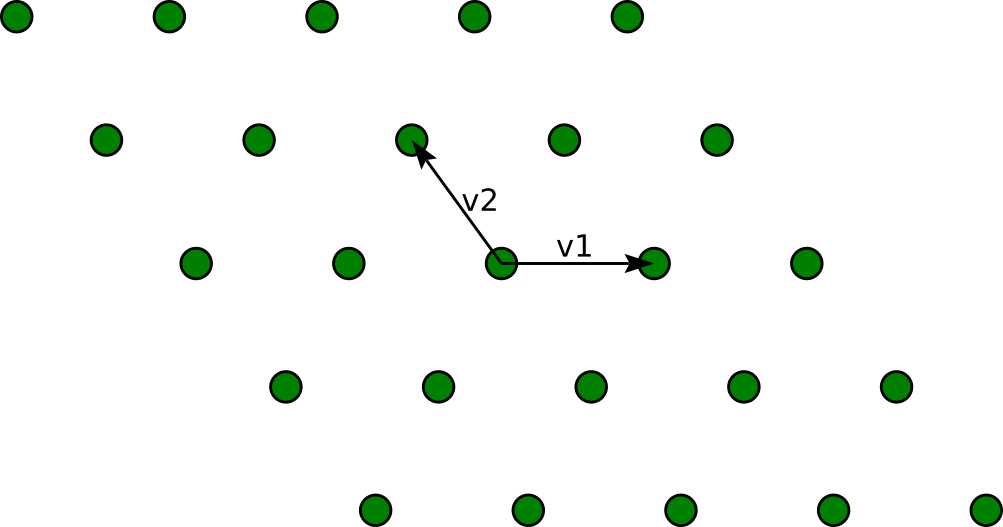
\includegraphics[width=0.6\textwidth]{./figures/lattice_basis.png}
	\caption{A 2-dimensional Bravais lattice.}
	\label{fig:lattice_basis}
\end{figure}
Figure \ref{fig:lattice_basis} shows a 2-dimensional lattice with basis vectors $\mathbf{v}_1$ and $\mathbf{v}_2$. Two Bravais lattices are considered equivalent if they are invariant under the same symmetry group. In 2 dimensions, there are 5 different Bravais lattices and in 3 dimensions, there are 14 \cite{kittel2005introduction}. The choice of a lattice basis for a certain Bravais lattice is not unique.
The Bravais lattice is invariant under translation by any of its basis vectors, meaning it is a periodic structure. 

Physical crystals also have an atomic basis consisting of a set of atoms and positions for these atoms. The atomic basis is repeated at each point on the underlying Bravais lattice and generates the physical crystal. A simple example is NaCl, which has a face-centred cubic Bravais lattice, and a 2 atom atomic basis.
\begin{figure*}[t!]
    \centering
    \begin{subfigure}[t]{0.5\textwidth}
        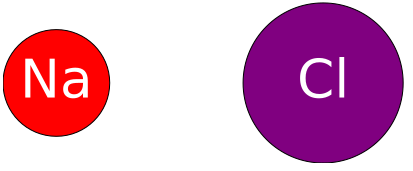
\includegraphics[width=0.7\textwidth]{./figures/na_cl_basis.png}
        \caption{The two basis atoms in NaCl}
	\label{fig:nacl_basis}
    \end{subfigure}%
    ~ 
    \begin{subfigure}[t]{0.5\textwidth}
        \centering
        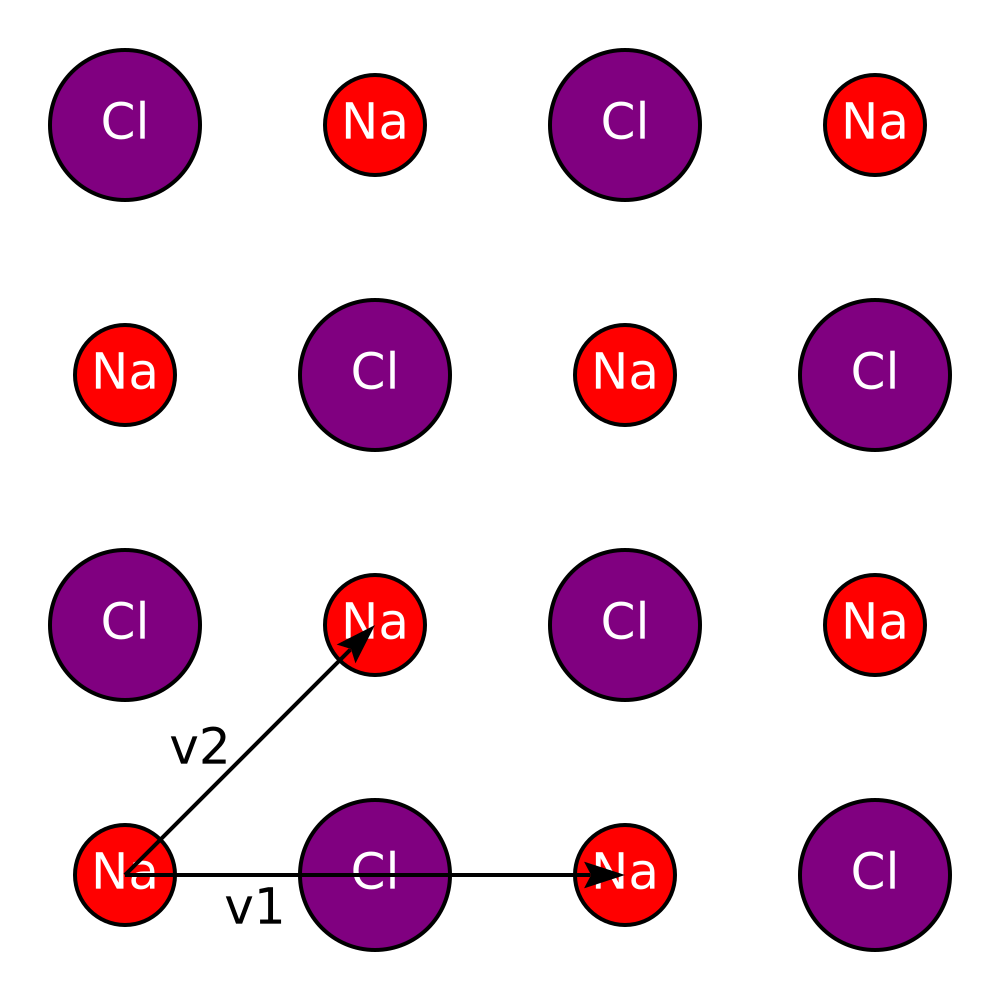
\includegraphics[width=0.6\textwidth]{./figures/na_cl_crosssection.png}
        \caption{A cross-section of the NaCl crystal, showing two of the three basis vectors}
	\label{fig:nacl_crosssection}
    \end{subfigure}
    \caption{NaCl atomic basis and crystal cross-section}
\end{figure*}

\subsection{Phonons}

\section{Methods}


\section{Results and Discussion}

\section{Conclusion}

\section{References}

% This command tells LaTeX how to format your references in the biblography. The standard plain formatting, with
% references appearing in the order they are cited, is absolutely fine for our needs.
\bibliographystyle{unsrt}

% This command includes the reference list. You will need to compile two or three times (perhaps BiBTeXing after
% the first time) to get the references in synch with the text.
\bibliography{ref}

% This command switches to appendices. The page count ends here.
% NOTE: the material contained in appendices will NOT count towards the assessment of your report.
% Consequently the main text should be self-contained.
\appendix

\end{document}
